\section{Conception du projet}
\begin{frame}{Les deux technologies}
\begin{description}
\item [Logoot] : Algorithme d'édition collaborative de documents dans un réseau
    Pair à Pair
  \begin{itemize}
    \item Développé par l'équipe GDD (Inria, LINA) ces dernières années
    \item Utilisé par le noyau pour faire l'édition collaborative
  \end{itemize} ~
\item [Criojo] : Langage de programmation \emph{chimique répartie}
  \begin{itemize}
    \item En cours de développement par l'équipe ASCOLA (Inria, LINA)
    \item Utilisé pour la distribution des modifications et la définition
    des documents
  \end{itemize}
\end{description}
\end{frame}

\begin{frame}{Logoot}
\begin{itemize}
  \item Gère les conflits d'édition dans un document distribué
  \item Génère des identifiants pour le partage des modifications entre les
  collaborateurs d'un document
  \item Analyse les identifiants reçus pour positionner les modifications dans
  le document
\end{itemize}
\end{frame}

\begin{frame}{Criojo}
Langage de programmation \emph{chimique répartie}
\begin{itemize}
  \item Définit des agents répartis qui consomment et produisent des messages
  sur le réseau.
  \item Représente l'état d'un agent comme une structure logique formée
  d'atomes.
\end{itemize}
\end{frame}

\begin{frame}{Criojo}
\begin{figure}
  \center
  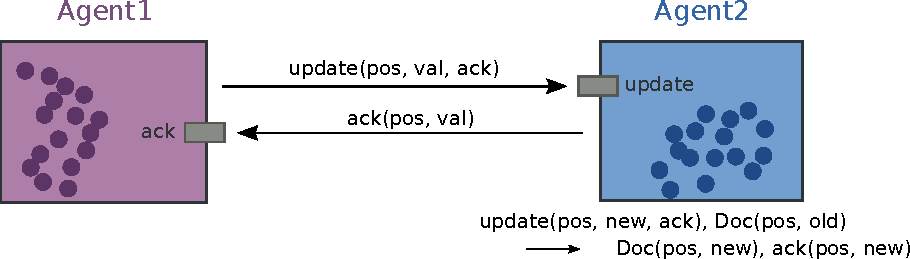
\includegraphics[width=.9\textwidth]{includes/criojo.pdf}
  \caption{Exemple Criojo}
\end{figure}
\end{frame}

\begin{frame}{État des lieux}
\begin{description}
  \item [Logoot]
  \begin{itemize}
    \item Projet de fin d'année de master sur l'implémentation de l'algorithme
    Logoot par des technologies web
    \item Projet encadré par Pascal Molli (GDD), l'un des concepteurs de Logoot
    \item Projet de 9 heures par semaines entre Janvier et Mars
  \end{itemize}~
  \item [Criojo]<2>
  \begin{itemize} 
    \item Stage de master sur le langage Criojo au sein de l'équipe ASCOLA :
    \begin{itemize} 
      \item Analyse et évolution du moteur chimique Criojo
      \item Implémentation de la communication entre agent (implémentation
      réalisée par un \emph{Message-Oriented Middleware} -- HornetQ)
      \item Implémentation d'un algorithme pour garantir la causalité
      (implémentation en cours, objectif fin Août) 
    \end{itemize}
    \item Stage de 5 mois
  \end{itemize}
\end{description}
\end{frame}

\begin{frame}{Ambition du projet}
\begin{itemize}
  \item Composer deux technologies provenant du monde de la Recherche
  \item \textbf{Pourquoi ?} Pour produire un programme ayant une utilité claire.
  Par exemple, à la fin du projet, avoir un plugin eclipse permettant de faire
  du code java de manière collaborative.
  \item \textbf{Comment ?} En utilisant les méthodes agiles (Scrum)
    \begin{itemize}
    \item Définir des cycles très courts de développement
    \item Fixer des réunions en fin de cycle avec un encadrant GDD, ASCOLA ou
    AtlanMod
    \end{itemize}
\end{itemize}
\end{frame}

